%%%%%%%%%%%%%%%%%%%%%%%%%%%%%%%%%%%
% Main Text
%%%%%%%%%%%%%%%%%%%%%%%%%%%%%%%%%%%

\textbf{ACKNOWLEDGMENT} \\ 
I would like to express my special thanks of gratitude to my teacher, Dr.Nguyen Viet Dung (dung.nguyenviet1@hust.edu.vn) who gave me the golden support to do this wonderful project. He gave a chance to use High GPU computing computer for AI Training. Otherwise, he also gave me recommendation on how to implement experiment to make a good conclusion such as what I should focus on, what I need to investigate, which metrics I should consider.\\

\textbf{ABSTRACT} \\
Today, the rapid development of industrial zones leads to an increasing incidence of skin diseases because of polluted air. According to a report by the American Cancer Society, it is estimated that in 2022 there will be about 100,000 people suffered from skin cancer and more than 7600 of these people will not survive. In the context that doctors at provincial hospitals and health facilities are overloaded, doctors at lower levels have lack of experience, having a tool to support doctors in the process of diagnosing skin diseases quickly and accurately is essential. Along with the strong development of artificial intelligence technologies, many solutions and tools to support the diagnosis of skin diseases have been researched and developed. These include DenseNet, InceptionNet, ResNet, NasNet, SeNet, EfficientNet, VGGNet. In this study, another approach to build tools to aid in the diagnosis of skin pathologies is proposed. SOTA (state of the art) models DenseNet, InceptionNet, ResNet, NasNet, MobileNet combined with Soft-Attention are used as backbone. In addition, personal information such as age and gender are also used. In addition, a new loss function that takes into account the imbalance of the data is also proposed. Experimental results on dataset HAM10000 show that using InceptionResNetV2 with Soft-Attetion and new loss function gives 90 percent accuracy, mean of precision, f1-score, recall-score, and auc- scores of 0.81, 0.81, 0.82, and 0.989, respectively, are improvements compared to published indexes. Besides, using MobileNetV3Large combined with Soft-Attention and new loss function, even though the number of parameters is 11 times less, the number of floors is 4 times less, it achieves 86 percent accuracy and 30 times faster diagnosis.\\
  
\section{Introduction}
\subsection{Problem Statement}
Skin cancer is one of the most common cancers leading to worldwide death. Every day, more than 9500\cite{03358} people in the United States are diagnosed with skin cancer. Otherwise, 3.6\cite{03358} million people are diagnosed with basal cell skin cancer each year. According to the Skin Cancer Foundation, the global incidence of skin cancer continues to increase\cite{11872}. In 2019, it is estimated that 192,310 cases of melanoma will be diagnosed in the United States\cite{11872}. On the other hand, if patients are early diagnosed, the survival rate is correlated with 99 percent. However, once the disease progresses beyond the skin, survival is poor\cite{11872}. Moreover, with the increasing incidence of skin cancers, low awareness among a growing population, and a lack of adequate clinical expertise and services, there is a need for effective solution. \\
Recently, deep learning particularly, and machine learning in general algorithms have emerged to achieve excellent performance on various tasks, especially in skin disease diagnosis tasks. AI-enabled computer-aided diagnostics (CAD) has solutions in three main categories: Diagnosis, Prognosis, and Medical Treatment. Medical imaging, including ultrasound, computed tomography, magnetic resonance imaging, and X-ray image is used extensively in clinical practice. In Diagnosis, Artificial Intelligence (AI) algorithms are applied for disease detection to save progress execution before these diagnosis results are considered by a doctor. In Prognosis, AI algorithms are used to predict the survival rate of a patient based on his/her history and medical data. In Medical Treatment, AI models are applied to building solutions for a specific disease, medicine revolution is an example. In various studies, AI algorithms have provided various end-to-end solutions in the detection of abnormalities such as breast cancer, brain tumors, lung cancer, esophageal cancer, skin lesions, and foot ulcers across multiple image modalities of medical imaging\cite{11872}. \\
In order to adapt the rise in skin cancer case, AI algorithms over the last decade has a great performance. Some typical models that can be mentioned are DenseNet\cite{06993}, EfficientNet\cite{04861}, Inception\cite{00567}, MobileNets\cite{04861}\cite{04381}\cite{02244}, ResNet\cite{03385}\cite{05027}, and NasNet\cite{07012}. Some of these models wich have been used as a backbone model in this paper will be discussed in the Related Work section. \\

\subsection{Literature Review}
Skin lesion classification is not a new area, since there are many great performance models constructed. One of the most cutting-edge technologies that have been used is Soft-Attention as stated in\cite{03358}. Soumyya and his team construct several models formed by the combination of a backbone model including DenseNet201\cite{06993}, InceptionResNetV2\cite{00567}, ResNet50\cite{03385}\cite{05027}, VGG16\cite{1556} and Soft-Attention layer. Using those above backbones has been tried by many previous papers including \cite{03798} which uses transfer learning approach with CNN based model, \cite{10348} which does not only use those above backbone model but also used InceptionV3\cite{00567} model. Another paper that uses the backbone models is \cite{09418}. Hemanth and his team decide to use EfficientNet\cite{11946} and SeNET\cite{01507} instead and CutOut\cite{04552v2} method which involves creating holes of different sizes on the images i.e. technically making a random portion of image inactive during data augmentation process. \cite{01284} also used Deep Convolution Neural Network. Moreover, that paper used RandArgument which crops an image into several images from a fixed size, DropBlock which is used for regularization, Multi-Weighted New Loss which is used for dealing with the imbalanced data problem, end-to-end Cumulative Learning Strategy which can more effectively balance representation learning and classifier learning without additional computational cost. Another state of the art is GradCam and Kernel SHAP\cite{06612}, which are both model agnostic, local interpretable methods that can highlight pixels that the trained network deems relevant for the final classification.\\
Otherwise, the Student and Teacher Model is also a state of the art in 2021\cite{03225}. The student and teacher model is the combination of two-mode which share the memory with each other. Therefore, they can take full advantage of what others learn. SkinLinkNet\cite{12602} and WonderM\cite{03426} are both tested the effect of segmentation on skin lesion classification problem. Another approach is using metadata including gender, age, and capturing position as stated in \cite{03910}. \\
On the other hand, skin lesion classification problems are not only applied by Deep Learning but also Machine Learning. Random Forest, XGBoost, and Support Vector Machines are tested by \cite{03798}. Besides, Isolation Forest is applied before the soft-max activation of the deep learning model to detect out of distribution skin lesion images as stated in\cite{10348}. Matrix Transformation, besides is also applied before the soft-max activation function in \cite{05045}. 

\subsection{Objectives}
In this paper, the effect of metadata on classifying skin disease is also analyzed .On the other hand, by analyzing the combination of several backbone models, I will also construct an optimized model that has the ability to classify in a balanced way between classes instead of well identifying the majority of classes. 

\section{Research Result}
\subsection{Data}
\subsubsection{Image Data}
The dataset used in this paper is the HAM10000 dataset published by Havard University Dataverse\cite{10417}. There are total 7 classes in this dataset containing Actinic keratoses and intraepithelial carcinoma or Bowen's disease (AKIEC), Basal cell Carcinoma (BCC),  benign keratosis-like lesions (solar lentigines / seborrheic keratoses andchen-planus like keratoses, BKL), dermatofibroma (DF), melanoma (MEL), melanocytic nevi (NV), and vascular lesions (angiomas, angiokeratomas, pyogenic granulomas and hemorrhage, VASC). The distribution of the dataset is shown in the table below:
\FloatBarrier
\begin{table}[ht]
	\centering
	\begin{tabular}{|c c c c c c c c c|} 
		\hline
		Class & AKIEC & BCC & BKL & DF & MEL & NV & VASC & Total \\ 
		\hline
		No. Sample & 327 & 514 & 1099 & 115 & 1113 & 6705 & 142 & 10015 \\
		\hline
	\end{tabular}
	\caption{Data Distribution in HAM10000}
	\label{table:1}
\end{table}
\FloatBarrier
\begin{figure}[h]
	\centering
	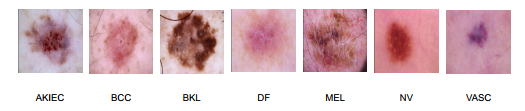
\includegraphics[width=1\linewidth]{img/DataDistribution}
	\caption{Example image of each class}
	\label{fig:datadistribution}
\end{figure}
More than 50 percent of lesions are confirmed through histopathology (HISTO), the ground truth for the rest of the cases is either follow-up examination (FOLLOWUP), expert consensus (CONSENSUS), or confirmation by in-vivo confocal microscopy (CONFOCAL). On the other hand, before being used for training the whole data is shuffled then split into two part. $90$ percent and $10$ percent of the data is used for training and validating respectively.\\
In the previous paper\cite{03358}, the image data is augmented for all class, the number of image increase to 18015 images. Since, this data is imbalanced, using augmented data may cause the problem of well classify on the majority of class. In this paper, instead of augmenting data, metadata is used. The way of processing metadata is discuss in MetaData section. Images in this dataset has the type of $RGB$ and shape of (450, 600). However, Each backbone need the different input size of image as well as the range of pixel value. DenseNet201\cite{06993} require the input pixels values are scaled between $0$ and $1$ and each channel is normalized with respect to the ImageNet dataset. In Resnet50 and Resnet152\cite{03385}\cite{05027}, the images are converted from $RGB$ to $BGR$, then each color channel is zero-centered with respect to the ImageNet dataset, without scaling. InceptionResNetV2\cite{11946}, on the other hand, will scale input pixels between $-1$ and $1$. Similarly, three versions of MobileNet\cite{04861}\cite{04381}\cite{02244}, NasNetMobile and NasNetLarge\cite{07012} require the input pixel is in range of $-1$ and $1$. 
\subsubsection{Metadata}
The HAM10000 dataset\cite{10417} also contain the metadata of patient including gender, age, and the capturing position. During the data exploration term, the age category miss 57 data point, which is decided to remove this 57 samples. In the gender and capturing position category contain some samples of unknown. Instead of removing, these unknowns data point is kept and considered as "prefer not to say". Besides, the label of the whole data is preprocessed into one-hot vector.
\subsection{Model Schema}
\subsubsection{Input Schema}
Using metadata as another input is not new. In paper\cite{03910}, they decide to keep the missing value and set its value to $0$. The sex and anatomical site are categorical encoded. The age, on the other hand is numerical normalized. After processing, the metadata is fed into a two-layer neural network with 256 neurons each. Each layer contains batch normalization, a ReLU\cite{08375} activation and dropout with $p = 0.4$. The network’s output is concatenated with the CNN’s feature vector after global average pooling. Especially, they use a simply data augmentation strategy to address the problem of missing values in metadata. During training, they randomly encode each property as missing with a probability of $p = 0.1$. \\
In this paper, the unknowns is kept as a type as discussed in Metadata section. Sex, anatomical site and age are also category encoded and numerical normalized, respectively. After processing, the metadata is then concatenated and fed into a dense layer of 4096 neurons. Finally, this this dense layer is then concatenate with the output of Soft-Attention which is then discussed in Soft-Attention section. \\
The Input schema is described as follow:\\
\begin{figure}[h]
	\centering
	\includegraphics[width=0.7\linewidth]{"Diagram/Input Schema"}
	\caption{Input Schema}
	\label{fig:input-schema}
\end{figure}\\
Image data, on the other hand after being preprocessed, is fed directly into the backbone model. 
\subsubsection{Soft-Attention}
Applying the Soft-Attention layer in deep learning is not a new approach. Soft-Attention has been used in various applications: image caption generation in \cite{03044} and handwriting verification in \cite{202017} respectively. In skin lesion classification, Soft-Attention is used to increase the performance of the model as described in \cite{03358}. Soft-Attention can ignore irrelevant areas of the image by multiplying the corresponding feature maps with low weights. The function below describes the flow of the Soft-Attention module:
\[
f_{sa} = \gamma t\sum_{k=1}^{K}softmax(W_k * t)
\]
In order to apply Soft-Attention, there are two main steps. Firstly, the input tensor is put in grid-based feature extraction from the high-resolution image, where each grid cell is analyzed in the whole slide to generate a feature map\cite{08513}. This feature map called $t \in R^{h \times w \times d}$ where $h, w, and d$ is the shape of tensor generated by a Convolution Neural Network(CNN), is then input to a 3D convolution layer whose weights is $W_k \in R^{h \times w \times d \times K}$. The output of this convolution is normalized using the softmax function to generate K = 16 attention maps. These $16$ attention maps are aggregated to produce a weight function called $\alpha$. This $\alpha$ function is then multiplied with feature tensor $t$ and scaled by $\gamma$, a learnable scalar. Finally, the out of Soft-Attention function $f_{sa}$ is the concatenation of the beginning feature tensor $t$ and the scaled attention maps. 
\begin{figure}[h]
	\centering
	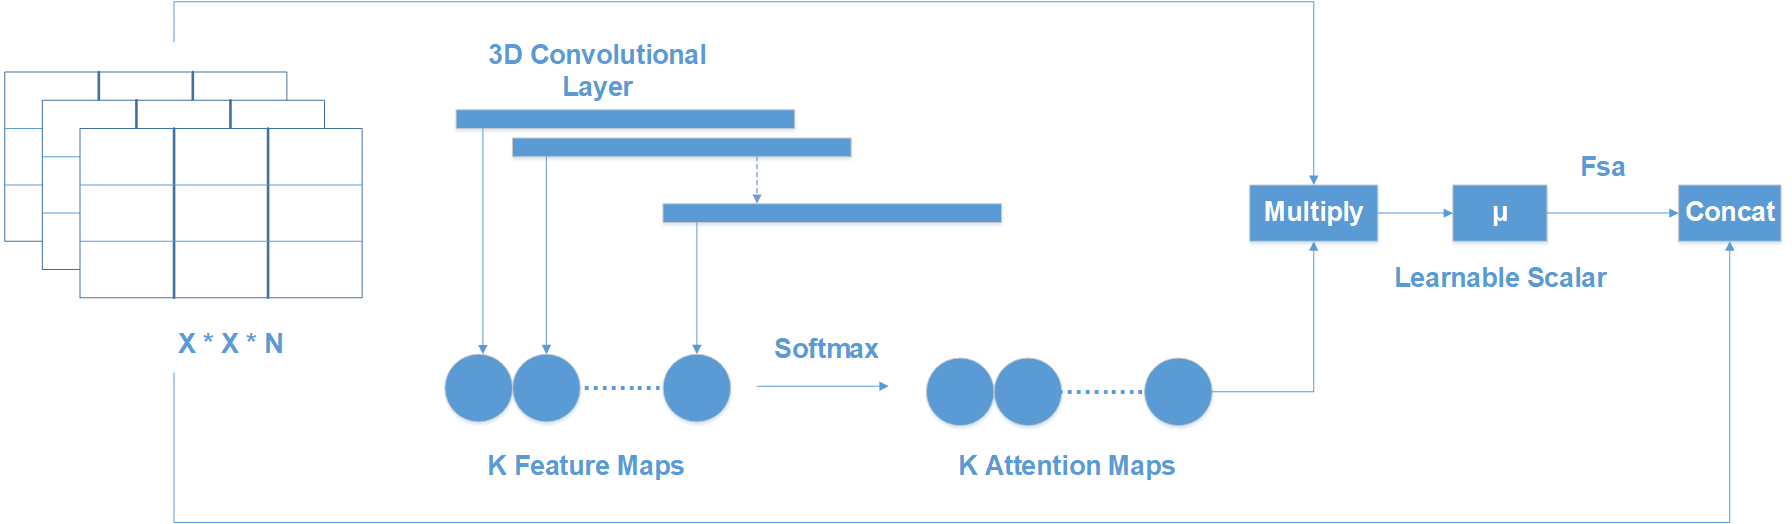
\includegraphics[width=1\linewidth]{Diagram/SoftAttention}
	\caption{Soft-Attention Module}
	\label{fig:softattention}
\end{figure}
In this paper, the Soft-Attention layer is applied in the same way in this paper\cite{03358}. The Soft-Attention module is described in the following diagram:
\begin{figure}[h]
	\centering
	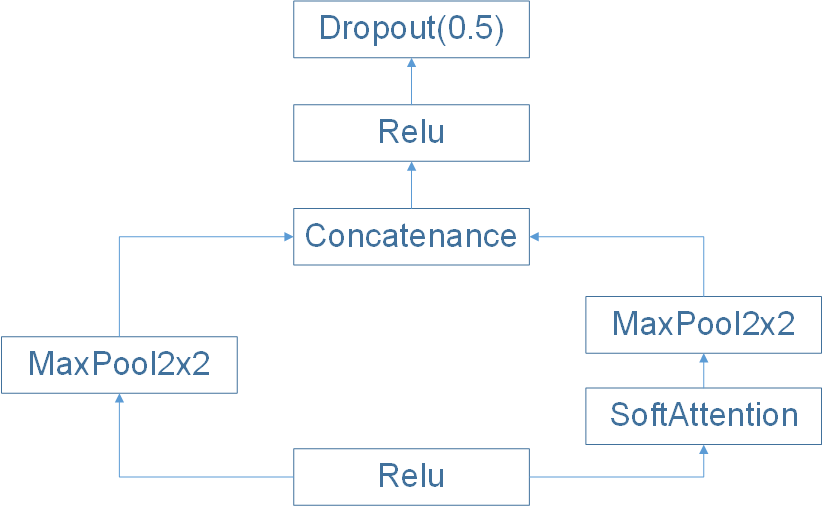
\includegraphics[width=0.5\linewidth]{Diagram/SoftAttentionBlock}
	\caption{Soft-Attention Module}
	\label{fig:softattentionblock}
\end{figure}\\

\subsubsection{Backbone Model Architecture}
In this paper, the backbone models that have been used are DenseNet201\cite{06993}, Inception\cite{00567}, MobileNets\cite{04861}\cite{04381}\cite{02244}, ResNet\cite{03385}\cite{05027}, and NasNet\cite{07012}. The combination of DenseNet201, InceptionResNetV2 and Soft-Attention layer are both tested by the previous paper\cite{03358} with a great performance. Otherwise, Resnet50 also well classify but with much less number of parameter and depth than based on its f1-score and precision stated. Therefore, in this paper, the performance of the model Resnet152 and NasnetLarge which has the larger number of parameter and depth is analyzed. On the other hand, three version of MobileNet and the NasnetMobile will also be analyzed which has a small number of parameter and depth.  
\FloatBarrier
\begin{table}[ht]
	\centering
	\begin{tabular}{|c | c c c|} 
		\hline
		Model & Size(MB) & Parameters & Depth \\ 
		\hline
		Resnet50 & 98 & 25.6M & 107 \\ 
		\hline
		Resnet152 & 232 & 60.4M & 311 \\ 
		\hline
		DenseNet201 & 80 & 20.2M & 402 \\
		\hline
		InceptionResNetV2 & 215 & 55.9M & 449 \\
		\hline
		MobileNet & 16 & 4.3M & 55 \\ 
		\hline
		MobileNetV2 & 14 & 3.5M & 105 \\ 
		\hline
		MobileNetV3Small & Unknown & 2.5M & 88 \\ 
		\hline
		MobileNetV3Large & Unknown & 5.5M & 118 \\
		\hline
		NasnetMobile & 23 & 5.3M & 308 \\
		\hline
		NasnetLarge & 343 & 88.9M & 533 \\ 
		\hline
	\end{tabular}
\caption{Size and Parameters and Depth of backbone model used in this paper}
\label{table:2}
\end{table}
\FloatBarrier

\subsubsection{Model}
The whole architecture of the model used for image feature extraction is applied in the same way in paper \cite{03358}. Metadata branch, otherwise is preprocessed before feeding into a dense layer then concatenate with the output of Soft-Attention layer. It is described in the figure below:
\begin{figure}[h]
	\centering
	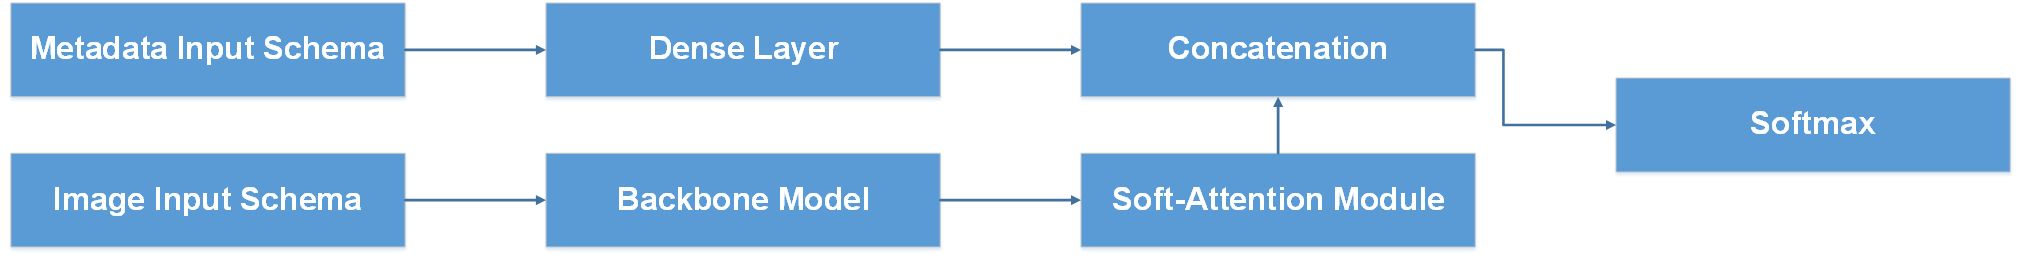
\includegraphics[width=1\linewidth]{Diagram/MainModel}
	\caption{Overall Model Architecture}
	\label{fig:mainmodel}
\end{figure}

\subsection{Loss Function}
The loss function used in this paper is categorical cross-entropy. Consider $X = [x_1, x_2, \dots, x_n]$ as the input feature, $\theta = [\theta_1, \theta_2, \dots, \theta_n]$. Let $N$, and $C$ is the number of training examples and number of class respectively. The categorical cross-entropy loss is presented as:
\[L(\theta, x_n) = -\frac{1}{N}\sum_{c=1}^{C}\sum_{n=1}^{N}W_c\times y^c_n \times \log(\hat{y}^c_n)\]
where $\hat{y}^c_i$  is the output of model and $y^c_i$ is the target that the model should return, $W_c$ is the weight of class $c$.\\
Since the dataset face the imbalanced problem then I applied the class weight for the loss. This formula below is used to calculate the class weight:
\[W = N \odot D\]
\[D = \begin{bmatrix}
	\frac{1}{C \times  N_1} & \frac{1}{C \times  N_2} & \dots & \frac{1}{C \times  N_n}\\
\end{bmatrix} = \frac{1}{C} \odot \begin{bmatrix}
\frac{1}{N_1} & \frac{1}{N_2} & \dots & \frac{1}{N_n}\\
\end{bmatrix}\]
where $N$ is the number of training sample, $C$ is the number of class, $N_i$ is the number of sample in each class $i$. $D$ is the matrix contain the inverse of $C \times N_i$. 
\subsection{Evaluation Metrics}
\begin{figure}[!htb]
	\begin{minipage}{0.48\textwidth}
		\centering
		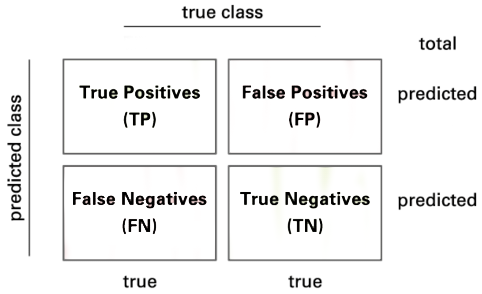
\includegraphics[width=1.1\linewidth]{img/Confusion-matrix}
		\caption{Confusion Matrix}\label{Fig:Data1}
	\end{minipage}\hfill
	\begin{minipage}{0.48\textwidth}
		\centering
		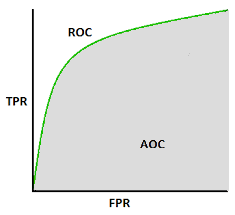
\includegraphics[width=.7\linewidth]{img/AUC}
		\caption{Area Under the Curve}\label{Fig:Data2}
	\end{minipage}
\end{figure}
In this paper, the model is evaluated by using the confusion matrix and related metrics. The figure 4 illustrates the presentation of a $2 \times 2$ confusion matrix used for $2$ class. Consider a confusion matrix $A$ with $C$ number of class. Let $A^i$ and $A^j$ is the set of $A$ rows and columns respectively. 
\[
	A = \begin{bmatrix}
		a_{11} & a_{12} & \dots & a_{1j} \\
		a_{21} & a_{22} & \dots & a_{2j} \\
		\vdots & \vdots	&  & \vdots\\
		a_{i1} & a_{i2} & \dots & a_{ij} 
	\end{bmatrix}
\]
The True Positive(TP) of all class in this case is the main diagonal of the matrix $A$. The following method are used to calculate the False Positives(FP), False Negatives(FN), and True Negatives(TN) of all class:
\[
	FP = -TP + \sum_{k=1}^{i}A^i_k \hspace{1cm} FN = -TP + \sum_{k=1}^{j}A^j_k
\]
\[
	TN_c = \sum_{i=1}^{C}\sum_{j=1}^{C}a_{ij} - \left[ \sum_{k=1}^{i}A^i_{i=c k} + \sum_{k=1}^{j}A^j_{j=c k} \right] + a_{i=c j=c} \implies TN = \begin{bmatrix}
		TN_1 & TN_2 & \dots & TN_c
	\end{bmatrix}
\]
Then, the model is evaluated by the following metrics:
\[\text{Sensitivity(Sens)} = \frac{TP}{TP + FN} \hspace{1cm} \text{Specificity(Spec)} = \frac{TN}{TN + FP}\]
\[\text{Precision} = \frac{TP}{TP + FP} \hspace{1cm} \text{F1 Score} = \frac{2 \times TP}{2 \times TP + FP + FN + TN}\]
\[\text{Accuracy} = \frac{TP + TN}{TP + FP + FN + TN} \hspace{1cm} \text{Balanced Accuracy} = \frac{\text{Sens} + \text{Spec}}{2}\]
The last metric is the $AUC$ score standing for Area Under the Curve which is the Receiver Operating Curve(ROC) that indicate the probability of TP versus the probability of FP.  
\subsection{Traning}
Before training, the dataset is split into three sub datasets including training, validation, and testing. In this paper, the graphic card that is used to train is Nvidia RTX TitanV.\\
All the model in this paper is trained with Adam Optimizer\cite{6980}. The initial learning rate is set to $0.001$, an learning rate reduction schedule is setup with the minimum learning rate is $0.0000001$ with the factor of $0.2$, the epsilon argument of the optimizer is set to $0.1$. On the other hand, Early Stopping is also set up, if the accuracy of validation set dose not increase after 25 epochs, the training will stop. 
\subsection{Results and Discusstion}
The accuracy of all model is presented in the figure below:
\FloatBarrier
\begin{table}[h]
	\centering
	\begin{tabular}{| c | c | c | c |}
		\hline
		InceptionResNetV2 & DenseNet201 & ResNet50 & VGG16 \\
		\hline
		0.93 & 0.91 & 0.92 & 0.88\\
		\hline
	\end{tabular}
\caption{Accuracy of the model with augmented data}
\label{table:3}
\end{table}
\FloatBarrier
\FloatBarrier
\begin{table}[h]
	\centering
	\begin{tabular}{| c | c | c | c | c |}
		\hline
		InceptionResNetV2 & DenseNet201 & ResNet50 & Resnet152 & MobileNetV2\\
		\hline
		0.89 & 0.89 & 0.70 & 0.57 & 0.81\\
		\hline
	\end{tabular}
\end{table}
\FloatBarrier
\FloatBarrier
\begin{table}[h]
	\centering
	\begin{tabular}{| c | c | c | c |}
		\hline
		MobileNetV3Large & MobileNetV3Small & NasNetLarge & NasNetMobile\\
		0.84 & 0.78 & 0.86 & 0.86\\
		\hline
	\end{tabular}
\caption{Accuracy of the model with metadata}
\label{table:4}
\end{table}
\FloatBarrier
According to the Table 3 and 4, it is clear that the model trained with augmented data has a higher accuracy than the model trained with metadata only. While InceptionResNetV2 and DenseNet201 trained with augmented data have accuracy of $0.93$ and $0.91$ respectively, their training with metadata has both the accuracy of $0.89$. Furthermore, Resnet50 trained with augmented data has the accuracy that outperform the Resnet50 and is twice as high as Resnet152 trained with metadata. On the other hand, mobile model including MobileNetV2, MobileNetV3Large, and NasNetMobile, even though has a much smaller number of parameters and depth than the other model, they have a quite good accuracy of $0.81$, $0.84$, $0.86$, respectively. This term will be discussed later on. Since, the model trained with augmented data have high accuracy, when their f1-score and the recall score of models are analyzed, it turns out that models trained with augmented data have imbalanced f1-scores according to table 5. As a results, augmented data model dose not classify well on all class as InceptionResNetV2 trained on augmented data have $0.29$ f1-score on class df while InceptionResNetV2 trained on metadata and the new weight loss can classify well in a balanced way. \\
\FloatBarrier
\begin{table}[h]
	\centering
	\begin{tabular}{|c | c | c | c | c | c | c | c | c|} 
		\hline
		Model & akiec & bcc & bkl & df & mel & nv & vasc & Mean \\
		\hline
		\thead{DenseNet201 +\\ Augmented Data} & 0.67 & 0.78 & 0.64 & 0.67 & 0.61 & 0.96 & 0.91 & 0.74 \\ 
		\hline
		\thead{InceptionResNetV2 +\\ Augmented Data} & 0.69 &	0.88 & 0.77 & 0.29 & 0.66 & 0.98 & 1 & 0.75\\
		\hline
		\thead{Resnet50 +\\ Augmented Data} & 0.53 & 0.86 & 0.68 & 0.67 & 0.57 & 0.97 & 0.95 & 0.74\\
		\hline 	
		\thead{VGG16 +\\ Augmented Data} & 0.65 & 0.7 & 0.52 & 0.4 & 0.53 & 0.95 & 0.95 & 0.67\\ 
		\hline		
		\thead{DenseNet201 +\\Metadata and WeightLoss} & \textbf{0.84} & 0.77 & \textbf{0.81} & \textbf{0.83} & \textbf{0.69} & 0.94 & 0.97 & \textbf{0.83}\\
		\hline
		\thead{InceptionResNetV2 +\\Metadata and WeightLoss} & 0.77 & 0.83 & \textbf{0.83} & 0.64 & \textbf{0.75} & 0.94 & 0.7 & \textbf{0.81}\\
		\hline
		\thead{Resnet50 +\\Metadata and WeightLoss} & 0.49 & 0.59 & 0.55 & 0.36 & 0.45 & 0.83 & 0.8 & 0.58\\
		\hline
		\thead{Resnet152 +\\Metadata and WeightLoss} & 0.42 & 0.38 & 0.41 & 0.15 & 0.4 & 0.75 & 0.75 & 0.46\\
		\hline
		\thead{MobileNetV2 +\\Metadata and WeightLoss} & 0.68 & 0.79 & 0.66 & 0.78 & 0.54 & 0.9 & \textbf{0.9} & 0.75\\
		\hline
		\thead{MobileNetV3Large +\\Metadata and WeightLoss} & 0.72 & 0.76 & 0.75 & 0.92 & 0.58 & 0.92 & \textbf{0.92} & 0.79\\
		\hline
		\thead{MobileNetV3Small +\\Metadata and WeightLoss} & 0.6 & 0.72 & 0.61 & 0.75 & 0.47 & 0.89 & \textbf{0.89} & 0.70\\
		\hline
		\thead{NasNetLarge +\\Metadata and WeightLoss} & 0.79 & 0.79 & 0.8 & 0.74 & 0.65 & 0.92 & 0.92 & \textbf{0.80}\\
		\hline
		\thead{NasNetMobile +\\Metadata and WeightLoss} & 0.76 & 0.74 & 0.78 & 0.73 & 0.63 & 0.93 & \textbf{0.93} & 0.78\\
		\hline
	\end{tabular}
	\caption{F1-Score of each class and the mean f1-score of each model}
	\label{table:5}
\end{table}
\FloatBarrier
However, only DenseNet201, InceptionResNetV2, and NasNetLarge whose depth are equal or larger than 400 have balanced f1-score on class. The others still face the imbalanced term. Since this dataset is not balanced, therefore using augmented data can make the model more  bias to the class which has larger sample. Using the metadata, though still make the model bias, it dose contributes to the improvement of  the performance of the model.\\ 
\FloatBarrier
\begin{table}[h]
	\centering
	\begin{tabular}{|l | c | c | c | c | c | c | c | c|} 
		\hline
		Model & akiec & bcc & bkl & df & mel & nv & vasc & Mean \\
		\hline
		\thead{DenseNet201 +\\ Augmented Data} & 0.52 & 0.77 & 0.58 & 0.5 & 0.71 & 0.97 & 1 & 0.72\\ 
		\hline
		\thead{InceptionResNetV2 +\\ Augmented Data} & 0.52 & 0.88 & 0.83 & 0.17 & 0.65 & 0.98 & 1 & 0.71\\
		\hline
		\thead{Resnet50 +\\ Augmented Data} & 0.43 & 0.85 & 0.7 & 0.5 & 0.47 & 0.98 & 0.9 & 0.69\\
		\hline 	
		\thead{VGG16 +\\ Augmented Data} & 0.61 & 0.81 & 0.44 & 0.44 & 0.68 & 0.95 & 0.9 & 0.69\\ 
		\hline		
		\thead{DenseNet201 +\\Metadata and WeightLoss} & \textbf{0.85} & 0.75 & 0.78 & 0.83 & 0.63 & 0.96 & \textbf{1} & \textbf{0.82}\\
		\hline
		\thead{InceptionResNetV2 +\\Metadata and WeightLoss} & \textbf{0.82} & 0.84 & 0.81 & 0.67 & 0.7 & 0.95 & 0.93 & \textbf{0.81}\\
		\hline
		\thead{Resnet50 +\\Metadata and WeightLoss} & 0.67 & 0.63 & 0.54 & 0.83 & 0.63 & 0.74 & 0.86 & 0.70\\
		\hline
		\thead{Resnet152 +\\Metadata and WeightLoss} & 0.51 & 0.49 & 0.35 & 0.76 & 0.47 & 0.63 & 0.48 & 0.52\\
		\hline
		\thead{MobileNetV2 +\\Metadata and WeightLoss} & 0.7 & 0.86 & 0.72 & 0.75 & 0.58 & 0.86 & \textbf{1} & 0.78\\
		\hline
		\thead{MobileNetV3Large +\\Metadata and WeightLoss} & 0.72 & 0.76 & 0.75 & \textbf{0.92} & 0.58 & 0.92 & 0.92 & \textbf{0.80}\\
		\hline
		\thead{MobileNetV3Small +\\Metadata and WeightLoss} & 0.76 & 0.84 & 0.68 & \textbf{1} & 0.52 & 0.82 & 0.93 & 0.79\\
		\hline
		\thead{NasNetLarge +\\Metadata and WeightLoss} & 0.73 & 0.71 & \textbf{0.83} & \textbf{0.92} & 0.59 & 0.9 & 0.93 & \textbf{0.81}\\
		\hline
		\thead{NasNetMobile +\\Metadata and WeightLoss} & \textbf{0.82} & 0.73 & \textbf{0.83} & \textbf{0.92} & 0.53 & 0.93 & 0.93 & \textbf{0.81}\\
		\hline
	\end{tabular}
	\caption{Recall score of each class and the mean recall score of each model}
	\label{table:6}
\end{table}
\FloatBarrier
This problem is also true with the recall score according to table 6. DenseNet201, InceptionResNetV2, ResNet50, VGG16 trained with augmented data has expected value of recall of $0.72$, $0.71$, $0.69$, $0.69$, respectively, while the combination of InceptionResNetV2, Metadata and the new weight loss function achieve the expected value of recall: $0.82$.
As the results, metadata does improve the model performance by reducing the amount of data needed for achieving nearly the expected results. On the other hand, the reason why the model become much more balanced is the weighted loss function. Weight loss function has ability to solve the imbalanced class samples by adding a weight related to the number of samples in each class. Therefore, DenseNet201, InceptionResNetV2 trained with the new weighted loss function have recall in akiec of $0.85$. $0.82$, respectively, as opposed to their training in akiec without weighted loss function. MobileV3large, MobileV3Small, NasNetLarge and NasNetMobile whose standard deviation is less than $0.15$ outperform others on classifying class df with the recall score of $0.92$, $1$, $0.92$, $0.92$, separately.\\ 
\begin{comment}
\FloatBarrier
\begin{table}[ht]
\centering
\begin{tabular}{|l | c | c | c | c | c | c | c|} 
\hline
Model & akiec & bcc & bkl & df & mel & nv & vasc \\
\hline
DenseNet201 + Augmented Data & 0.96 & 0.98 & 0.9 & 0.80 & 0.95 & 0.95 & 0.999\\ 
\hline
InceptionResNetV2 + Augmented Data & 0.96 & 0.99 & 0.96 & 0.92 & 0.97 & 0.976 & 0.999\\
\hline
Resnet50 + Augmented Data & 0.97 & 0.99 & 0.91 & 0.94 & 0.95 & 0.95 & 0.99\\
\hline 	
VGG16 + Augmented Data & 0.98 & 0.99 & 0.96 & 0.97 & 0.97 & 0.97 & 0.99\\ 
\hline		
DenseNet201 + Metadata & 0.99 & 0.99 & 0.97 & 0.99 & 0.92 & 0.96 & 0.99\\
\hline
InceptionResNetV2 + Metadata & 0.98 & 0.98 & 0.98 & 0.98 & 0.95 & 0.96 & 0.99\\
\hline
Resnet50 + Metadata & 0.97 & 0.95 & 0.88 & 0.99 & 0.85 & 0.92 & 0.98\\
\hline
Resnet152 + Metadata & 0.95 & 0.9 & 0.84 & 0.92 & 0.82 & 0.89 & 0.8\\
\hline
MobileNetV2 + Metadata & 0.97 & 0.98 & 0.94 & 0.99 & 0.9 & 0.95 & 0.99\\
\hline
MobileNetV3Large + Metadata & 0.99 & 0.98 & 0.96 & 0.99 & 0.92 & 0.95 & 0.99\\
\hline
MobileNetV3Small + Metadata & 0.97 & 0.97 & 0.93 & 0.99 & 0.87 & 0.94 & 0.99\\
\hline
NasNetLarge + Metadata & 0.95 & 0.98 & 0.97 & 1 & 0.92 & 0.95 & 1\\
\hline
NasNetMobile + Metadata & 0.98 & 0.99 & 0.97 & 1 & 0.9 & 0.96 & 1\\
\hline
\end{tabular}
\caption{ROC AUC Score of each model}
\label{table:7}
\end{table}
\FloatBarrier
\end{comment}
Another interesting point found during the experiment is that MobileNetV2, MobileNetV3 and NasNetMobile have small number of parameters and depth, though have relative good performance. The table 8 illustrates the deeper analyzing of the three models. It's clear that MobileNetV3Large and NasNetMobile are the two best performance model.
\FloatBarrier
\begin{table}[ht]
	\centering	
	\begin{tabular}{|l | c | c | c | c|} 
		\hline
		Model & \cite{04381} & \cite{02244}Small & \cite{02244}Large & \cite{07012}Mobile\\
		\hline
		Accuracy(avg) & 0.81 & 0.78 & 0.84 & \textbf{0.86}\\
		\hline
		Balanced Accuracy(avg) & 0.86 & 0.87 & 0.87 & \textbf{0.88}\\ 
		\hline
		Precision(avg) & 0.71 & 0.63 & \textbf{0.75} & 0.73\\
		\hline
		F1-score(avg) & 0.75 & 0.70 & \textbf{0.79} & 0.78\\
		\hline
		Sensitivity(avg) & 0.78 & 0.79 & 0.80 & \textbf{0.81}\\ 
		\hline
		Specificity(avg) & 0.95 & 0.95 & 0.95 & \textbf{0.96}\\
		\hline
		ROC-AUC-score(avg) & 0.96 & 0.95 & 0.96 & \textbf{0.97}\\
		\hline
	\end{tabular}
	\caption{Deeper analyzing of mobile model}
	\label{table:8}
\end{table}
\FloatBarrier
Nevertheless, MobileNetV3Large has less number of parameters and depth than NasNetMobile according to the table 2. Therefore, at the end of this experiment, I decide to configure the MobileNetV3Large to construct an optimized model. The result of this experiment is illustrated in table 9.
\FloatBarrier
\begin{table}[ht]
	\centering
	\begin{tabular}{|l | c |}
		\hline
		Model & Accuracy\\
		\hline
		MobileNetV3Large-Layer[:270] + Soft-Attention + Metadata & 0.71 \\
		\hline
		MobileNetV3Large-Layer[:266] + Soft-Attention + Metadata  & 0.73 \\
		\hline
		MobileNetV3Large-Layer[:260] + Soft-Attention + Metadata  & 0.77 \\
		\hline
		MobileNetV3Large-Layer[:251] + Soft-Attention + Metadata  & 0.79 \\
		\hline
		MobileNetV3Large-Layer[:246] + Soft-Attention + Metadata  & 0.84 \\
		\hline
		MobileNetV3Large-Layer[:246] + Soft-Attention + Dense(512) + Metadata & 0.85 \\
		\hline
		MobileNetV3Large-Layer[:240] + Soft-Attention + Metadata  & \textbf{0.86}\\
		\hline
		MobileNetV3Large-Layer[:230] + Soft-Attention + Metadata  & 0.84 \\
		\hline
		MobileNetV3Large-Layer[:230] + Soft-Attention & 0.85 \\ 
		\hline
		MobileNetV3Large & 0.85 \\ 
		\hline
	\end{tabular}
	\caption{Deeper analyzing of MobileNetV3Large Model}
	\label{table:9}
\end{table}
\FloatBarrier
The Table 9 demonstrate that the Soft-Attention and the metadata have a good effect on the model. Otherwise, Adding a dense layer does not increase the model performance. The best MobileNetV3Large model architecture is the combination of MobileNetV3Large replaced from $241^{th}$ layer to the rest by Soft-Attention layer and the metadata, which peak the model performance of $0.86$ accuracy rate. 
\FloatBarrier
\begin{table}[ht]
	\centering
	\begin{tabular}{| l | c |}
		\hline
		Accuracy & 0.86\\
		\hline
		Precision(avg) & 0.86\\
		\hline
		F1-score(avg) & 0.86\\
		\hline
		Sensitivity(avg) & 0.86\\
		\hline
		Specificity(avg) & 0.95\\
		\hline
		ROC AUC Score(avg) & 0.98\\
		\hline
	\end{tabular}
	\caption{Performance of MobileNetV3Large}
	\label{table:10}
\end{table}
\FloatBarrier
\begin{table}[ht]
	\centering
	\begin{tabular}{| l | c | c | c |}
		\hline
		Model & MobileNetV3Large & DenseNet201 & InceptionResnetV2\\
		\hline
		No. Parameters & \textbf{5.5M} & 20.2M & 55.9M\\
		\hline
		Depth & \textbf{118} & 402 & 449\\
		\hline
		Accuracy & 0.86 & 0.89 & 0.90\\
		\hline
		Time Prediction(s/epochs) & \textbf{116} & 1000 & 3500 \\
		\hline
	\end{tabular}
\caption{How Performance of MobileNetV3Large be optimized}
\label{table:11}
\end{table}
\FloatBarrier
\section{Conclusion}
In this paper, my objective is to analyze the effect of metadata on the performance of model as well as identifying whether metadata can make the model less imbalanced or not. On the other hand, I also try to construct an optimized and balanced model that can be used on mobile phone or electronic devices. The experiment shown that metadata improve the model performance, the factor that make the model much more imbalanced is the augmented data. This problem can be solve quite absolutely by using aforementioned weighted loss function. Using weighted loss function make the expected value of model f1-score increase. At the end of the experiment, mobile model is found that can achieve great performance without either the large number of parameters or depth.  
\clearpage
\pagebreak

